\section{Experimental Results}

\textcolor{red}{(TODO: performance results are not included in section 6. we
should add some numbers such as runtime, throughput, cdf of latency, and SW
overhead)}

We have implemented \textsf{PCStream} on the Linux kernel 4.5 that runs on
Intel's i7-2600 CPUs with 8 cores and with 16~GB DRAM.  Samsung's PM963 480~GB
SSD with a multi-stream feature is used.  PM963 supports up to 9 streams; 8
user-configurable streams and one default stream. Write requests that do not
specify their stream IDs are assigned the default stream.  To support the
internal stream, we have modified the SSD firmware.  For detailed performance
analysis, an \texttt{nvme-cli} tool is modified to retrieve the information of
\textsf{PCStream}-enabled device internals, such as the WAF or
\textcolor{red}{the valid time of data in every blocks}.

%and its firmware has been modified to
%support the internal stream.

For an objective evaluation, we compared \textsf{\small PCStream} with three
existing schemes: \textsf{\small Baseline}, \textsf{\small
ManualStream}~\cite{MultiStream}, and \textsf{\small
AutoStream}~\cite{AutoStream}.  \textsf{\small Baseline} stands for a legacy
SSD that does not support multiple streams. \textsf{\small ManualStream}
represents multi-streamed SSDs with manual stream allocation.  \textsf{\small
AutoStream} is one that employs an LBA-based data separation technique which is
implemented at the device driver layer. 

We have carried out experiments with various benchmark programs, including
RocksDB~\cite{}, Cassandra~\cite{}, SQLite~\cite{}, and GCC~\cite{}, each of
which generates distinct write patterns.  RocksDB and Cassandra have
append-only write patterns; SQLite has in-place update write patterns; GCC has
write-once patterns.  We also run the combinations of multiple programs
simultaneously for assessments under more realistic environments.  Yahoo! Cloud
Serving Benchmark (YCSB)~\cite{YCSB} with 120,000,000 keys runs on top of
RocksDB and Cassandra.  Both RocksDB and Cassandra are based on the LSM-tree
algorithm, so they have three major I/O activities (e.g.,
\textcolor{red}{logging, flush, and compaction}) as analyzed in Section 3.
%However, we identified about 5 PCs during runtime and we consider the extra
%PCs as management use.
TPC-C~\cite{TPCC} runs on SQLite with 20 warehouses.  Similarly, SQLite has two
major I/O activities (e.g., \textcolor{red}{logging and YYY}). 
%2 kinds of data types in theory but we identified 4 PCs.
GCC compiles kernel source code 30 times. For the each run, 1/3 of source files
that are randomly chosen are modified and involved in the compilation.  GCC
creates many temporary files (e.g., \textcolor{red}{XXX}) as well as long-lived
files (e.g., \textcolor{red}{YYY}), thereby having more than 20 PCs.  To
generate mixed workloads, we run RocksDB and GCC scenarios together (denoted by
Mixed 1), and run SQLite and GCC scenarios at the same time (denoted by Mixed
2).
%Since GCC writes many kinds of temporary files as well as long-lived files,
%GCC has more than 20 PCs which makes clustering process effective for the GCC
%and mixed workloads.
To emulate an aged SSD, 90\% of the total SSD capacity was initially filled up
with user files before benchmarks run.


\subsection{WAF Comparison}

\begin{figure}[t]
	\centering
	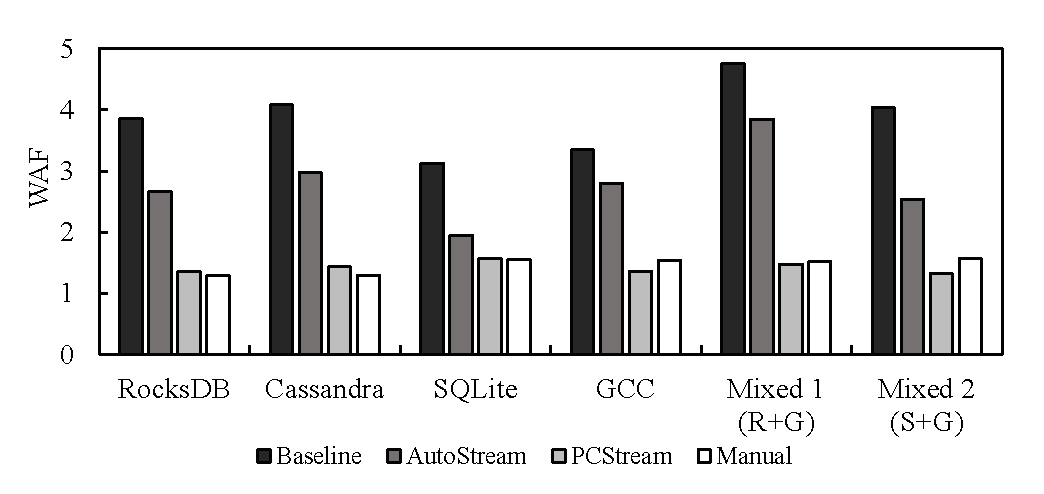
\includegraphics[width=0.9\linewidth]{figure/waf}
	\caption{The WAF comparison for various workloads.}
	\label{fig:waf}
	%\vspace{-36pt}
\end{figure}

We compared WAF of the existing techniques with \textsf{PCStream} for various
workloads, and the result is shown in Fig.~\ref{fig:waf}.  Overall,
\textsf{PCStream} was as efficient as \textsf{Manual}; Across all the
benchmarks, \textsf{PCStream} showed quite similar WAF values as
\textsf{Manual}. \textsf{PCStream} reduced WAF values by 63\% and 49\% over
\textsf{Baseline} and \textsf{AutoStream}, respectively, on average.  The
result shows that separating short-lived data (e.g., log or temp files) from
long-lived one (e.g., compaction or result files) using PC was quite effective.

As expected, \textsf{Baseline} showed the worst performance among all the
techniques.  We also observed that AutoStream was not able to achieve high WAF
reduction.  This was because the lack of relationship between hotness of data
and LBAs. Except for SQLite, all other benchmarks wrote data in an append-only
and/or a write-only manner. Since \textsf{PCStream} and \textsf{Manual} did not
depend upon LBAs for hot-cold separation, they performed well consistently,
regardless of write access patterns.


%Only SQLite had in-place update patterns for log files, 
%but the larger amount of data were written to database files 
%whose lifetimes are determined by the client
%which makes hard to predict their lifetime by the address.  In PCStream,
%however, long-lived data in database files are moved to internal streams during
%GC so that we can further reduce WAF.

One of the noticeable observations in Fig.~\ref{fig:waf} was that PCStream
performed even better than Manual for GCC, Mixed 1, and Mixed 2.  Those
benchmarks created many streams larger than ones supported by PM963.  In
\textsf{Manual}, application code was manually annotated at offline, so that
write I/Os from specific routines were assigned to designated SSD stream IDs.
Hence, it is impossible to know which applications run simultaneously, how many
streams would be created by them, and how to map those streams to SSD streams
in an optimal manner. Consequently, assigned stream IDs cannot be changed or
adjusted at run time adapting to the characteristics of programs running.
Unlike \textsf{Manual}, \textsf{PCStream} collected all PCs at run time,
clustered, and assigned them to SSD stream IDs, thereby outperforming
\textsf{Manual}.

%since the Manual scheme has static stream allocation.
%In Manual, once data types is mapped to the stream, the mapping is not changed 
%during runtime.
%For complex workloads which have large number of PCs such as mixed cases,
%it is difficult to expect data lifetimes in detail based on the data types.
%If the lifetime pattern is changed during runtime or the programmer choose
%second best stream mapping,
%Manual scheme lose the potential benefit in reducing WAf.
%However, the reclustering enables PCStream to adapt changing workload or find
%better stream mapping.
%The detailed analysis will be shown in the following subsections.

\begin{comment}
For example, both \textsf{\small PCStream} and \textsf{\small Manual} reduced WAF by 38\% over \textsf{\small Baseline} for the \texttt{UR} case. 
Compared with \textsf{\small AutoStream}, \textsf{\small PCStream} was more effective, reducing WAF more by 35\% on average.  
\textsf{\small PCStream} outperformed \textsf{\small AutoStream} by reducing WAF by 35\% on average.
Fig. 6 also indicates that the two-phase stream assignment technique is effective.  
\textsf{\small PCStream} outperformed \textsf{\small PCStream$^{*}$} by 12\% on average in the WAF reduction.
As shown in Fig. 6, \textsf{\small PCStream$^*$} reduced WAF by up to 30\% over \textsf{\small AutoStream}.  
\end{comment}

\subsection{Per-stream Lifetime Distribution Analysis}

\begin{figure}[t]
	\centering
	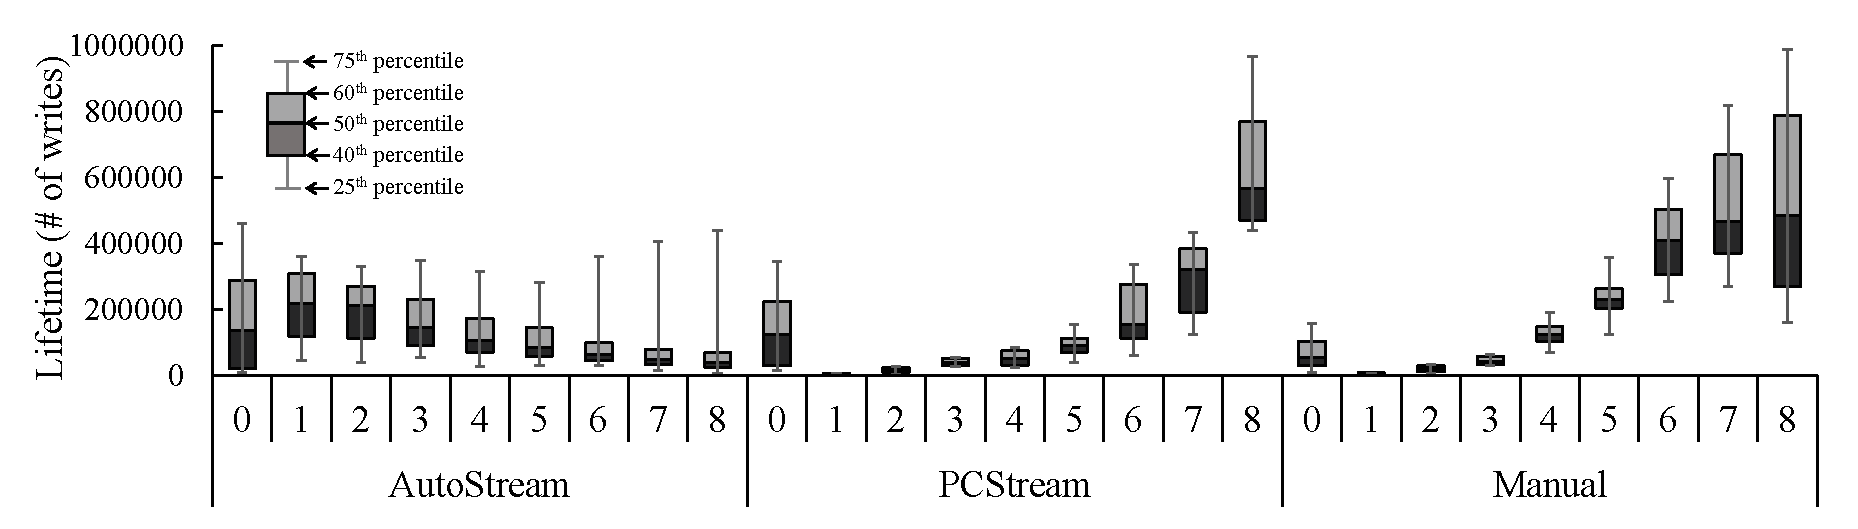
\includegraphics[width=1\linewidth]{figure/distribution}
	\caption{A Comparison of lifetime distributions of the smaller variance streams.}
	\label{fig:distribution}
	%\vspace{-36pt}
\end{figure}

To better understand the benefit of \textsf{\small PCStream} on WAF reduction,
we measured per-stream lifetime distributions for the \texttt{Mixed 1}
scenario.  Fig.~\ref{fig:distribution} shows a box plot of data lifetimes from
the 25th to the 75th percentile.  As shown in Fig.~\ref{fig:distribution},
streams in both \textsf{\small PCStream} and Manual are roughly categorized as
two groups, $G1$ = $\{$1, 2, 3, 4, 5$\}$ and $G2$ = $\{$6, 7, 8$\}$, where $G1$
includes streams with short lifetimes and small variances (i.e., streams 1, 2,
3, 4, and 5) and $G2$ includes streams with large lifetimes and large variances
(i.e., streams 6, 7, and 8). The stream 0 does not belong to any groups as it
is assigned to requests whose lifetimes are unknown.  Even though the variance
in the stream 0 is wider than that in Manual, PCStream showed similar
per-stream distributions as Manual. In particular, for the streams in $G2$,
PCStream exhibited smaller variance than Manual, which means that PCStream
separates cold data from hot data efficiently.

AutoStream was not able to achieve small variance of data lifetimes in
comparison with PCStream and Manual. At first, AutoStream assigns data to the
stream 0 and then increases the stream number according to their update
frequency. In Fig.~\ref{fig:distribution}, we found that short-lived data were
generally allocated to higher streams.  However, high variance observed across
all the streams indicates hot data are often mixed up with cold one.  This is
an expected result. In RocksDB and GCC workloads, there is no strong relation
between hotness of data and LBA.  Thus, long-lived data are often written to
LBAs where short-live data were previously written to, and it results in very
high lifetime variances for all the streams.

\subsection{Impact of the Internal Stream}

In order to understand the impact of the two-phase assignment, we compared each
technique with and without the internal stream.  The internal stream works
independently of a stream assignment method running at the host level, so it
can easily be combined with any host-level techniques.  Fig.~\ref{fig:internal}
shows a comparison of WAF values of Baseline, AutoStream, and PCStream under
the five workloads.  At a glance, we notice that all the techniques benefited
from using the internal stream.  However, its impact was not so high to offset
WAF costs caused by the improper stream assignment by the first-phase.  For
example, in Baseline, all the data from the host are first written to the same
default stream, regardless of their hotness.  Then, during SSD GC, cold data
that are left valid in the default stream are moved to the internal stream.
This helps us prevent cold data from being mixed up with future incoming data,
separating hot and cold data in two different segments. However, since the host
keeps writing the mixture of hot/cold data to the default stream, it is
impossible to avoid extra copy costs involved in the default stream.
AutoStream worked better than Baseline by assigning hot and cold data to
different streams, but owing to the inaccuracy of LBA-based hot-cold detection,
it performed worse than PCStream.

\begin{figure}[t]
	\centering
	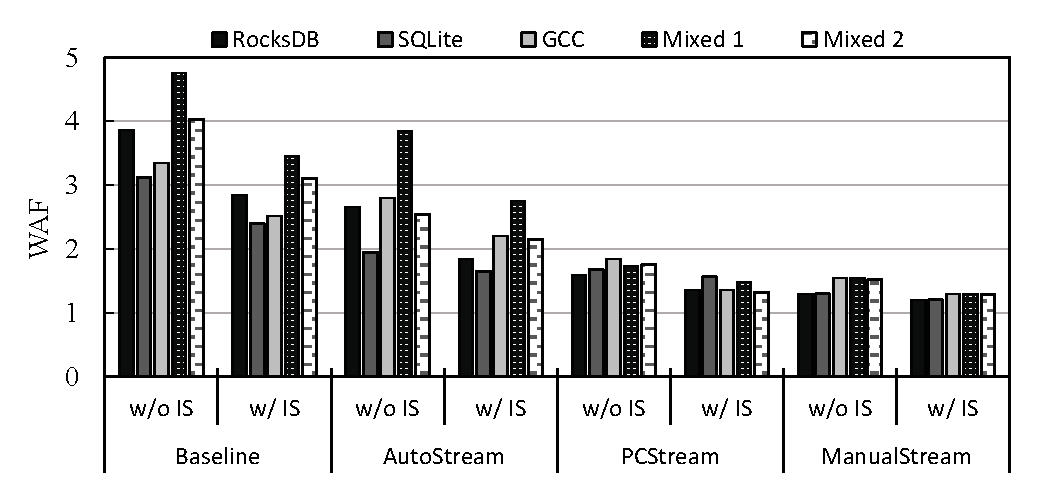
\includegraphics[width=0.9\linewidth]{figure/internal}
	\caption{Comparison of WAF w/ and w/o internal streams.}
	\label{fig:internal}
	%\vspace{-36pt}
\end{figure}


\subsection{Impact of the PC-stream table}

\begin{figure}[t]
	\centering
	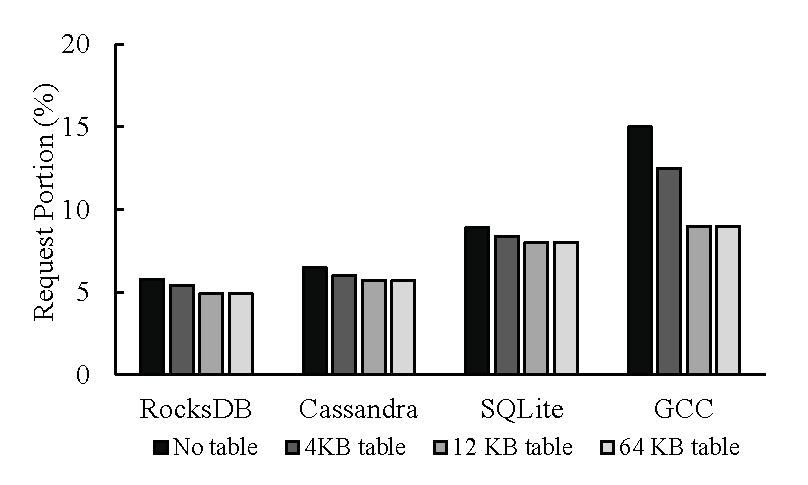
\includegraphics[width=0.7\linewidth]{figure/pctable}
	\caption{Request portion comparison of stream 0 with PC-stream table.
		\textcolor{red}{
			(TODO: How about adding the size of PC-stream table? It was mentioned in
			the text of the paper.)}
		}
	\label{fig:pctable}
	%\vspace{-36pt}
\end{figure}

As explained in Section 5, the PC-stream table provides us with a long-term
history of applications' I/O behaviors, and it even works for short-lived
applications that are frequently launched and terminated. To confirm its
benefits, we have modified \textsf{PCStream} so that it throws away the
contents of the PC-stream table at the end of each benchmark runs. For example,
in the kernel compilation scenario with GCC, the PC-stream table is
intentionally set empty after each run finishes, and thus the next run will
start without any prior knowledge about past PCs.

Fig.~\ref{fig:pctable} illustrates our experimental results, which shows how
many requests are sent to the stream 0. In \textsf{PCStream}, the stream 0 is
assigned to write requests whose lifetime behaviors are not estimated yet.
Therefore, the more write requests are assigned to the stream 0, the less the
history \textsf{PCStream} maintains. As shown in Fig.~\ref{fig:pctable}, in
RocksDB, Cassandra, and SQLite, the absence of the PC-stream table did not
affect the number of requests send to the stream 0. This is because those
programs ran continuously for a long time. Unlike them, GCC involves frequent
creations and termination of processes (\textit{e.g.}, \textcolor{red}{XXX}).
Hence, without the PC-stream table, about 16\% of requests were sent to the
stream 0. With the PC-stream table, it was reduced to less 10\%. We also
observed that with, the PC-stream table, the WAF value was reduced from 1.96 to
1.54 for GCC.

